\documentclass{report}
% Include all project wide packages here.
\usepackage{fullpage}
\usepackage[style=ieee]{biblatex}
\usepackage[dutch]{babel}

\renewcommand{\familydefault}{\sfdefault}

\setmainfont[Ligatures=TeX]{Myriad Pro}
\setmathfont{Asana Math}
\setmonofont{Lucida Console}

\usepackage{titlesec, blindtext, color}
\definecolor{gray75}{gray}{0.75}
\newcommand{\hsp}{\hspace{20pt}}
\titleformat{\chapter}[hang]{\Huge\bfseries}{\thechapter\hsp\textcolor{gray75}{|}\hsp}{0pt}{\Huge\bfseries}
\renewcommand{\familydefault}{\sfdefault}
\renewcommand{\arraystretch}{1.2}
\setlength\parindent{0pt}

%For code listings
\definecolor{black}{rgb}{0,0,0}
\definecolor{browntags}{rgb}{0.65,0.1,0.1}
\definecolor{bluestrings}{rgb}{0,0,1}
\definecolor{graycomments}{rgb}{0.4,0.4,0.4}
\definecolor{redkeywords}{rgb}{1,0,0}
\definecolor{bluekeywords}{rgb}{0.13,0.13,0.8}
\definecolor{greencomments}{rgb}{0,0.5,0}
\definecolor{redstrings}{rgb}{0.9,0,0}
\definecolor{purpleidentifiers}{rgb}{0.01,0,0.01}


\lstdefinestyle{csharp}{
language=[Sharp]C,
showspaces=false,
showtabs=false,
breaklines=true,
showstringspaces=false,
breakatwhitespace=true,
escapeinside={(*@}{@*)},
columns=fullflexible,
commentstyle=\color{greencomments},
keywordstyle=\color{bluekeywords}\bfseries,
stringstyle=\color{redstrings},
identifierstyle=\color{purpleidentifiers},
basicstyle=\ttfamily\small}

\lstdefinestyle{c}{
language=C,
showspaces=false,
showtabs=false,
breaklines=true,
showstringspaces=false,
breakatwhitespace=true,
escapeinside={(*@}{@*)},
columns=fullflexible,
commentstyle=\color{greencomments},
keywordstyle=\color{bluekeywords}\bfseries,
stringstyle=\color{bluestrings},
identifierstyle=\color{purpleidentifiers}
}

\lstdefinestyle{vhdl}{
language=VHDL,
showspaces=false,
showtabs=false,
breaklines=true,
showstringspaces=false,
breakatwhitespace=true,
escapeinside={(*@}{@*)},
columns=fullflexible,
commentstyle=\color{greencomments},
keywordstyle=\color{bluekeywords}\bfseries,
stringstyle=\color{redstrings},
identifierstyle=\color{purpleidentifiers}
}

\lstdefinestyle{xaml}{
language=XML,
showspaces=false,
showtabs=false,
breaklines=true,
showstringspaces=false,
breakatwhitespace=true,
escapeinside={(*@}{@*)},
columns=fullflexible,
commentstyle=\color{greencomments},
keywordstyle=\color{redkeywords},
stringstyle=\color{bluestrings},
tagstyle=\color{browntags},
morestring=[b]",
  morecomment=[s]{<?}{?>},
  morekeywords={xmlns,version,typex:AsyncRecords,x:Arguments,x:Boolean,x:Byte,x:Char,x:Class,x:ClassAttributes,x:ClassModifier,x:Code,x:ConnectionId,x:Decimal,x:Double,x:FactoryMethod,x:FieldModifier,x:Int16,x:Int32,x:Int64,x:Key,x:Members,x:Name,x:Object,x:Property,x:Shared,x:Single,x:String,x:Subclass,x:SynchronousMode,x:TimeSpan,x:TypeArguments,x:Uid,x:Uri,x:XData,Grid.Column,Grid.ColumnSpan,Click,ClipToBounds,Content,DropDownOpened,FontSize,Foreground,Header,Height,HorizontalAlignment,HorizontalContentAlignment,IsCancel,IsDefault,IsEnabled,IsSelected,Margin,MinHeight,MinWidth,Padding,SnapsToDevicePixels,Target,TextWrapping,Title,VerticalAlignment,VerticalContentAlignment,Width,WindowStartupLocation,Binding,Mode,OneWay,xmlns:x}
}

%defaults
\lstset{
basicstyle=\ttfamily\small,
extendedchars=false,
numbers=left,
numberstyle=\ttfamily\tiny,
stepnumber=1,
tabsize=4,
numbersep=5pt
}
\addbibresource{../../library/bibliography.bib}

\title{EPO-2: Mid-term Design Report - Draadloze communicatie met zigBee module}
\author{Tijmen Witte}

\begin{document}

\chapter{Draadloze communicatie met ZigBee module}
\label{ch: draadloze communicatie met ZigBee module}

Een van de opdrachten van het project is om de robot te begeleiden via een C-programma.
Het is de bedoeling dat we door middel van het draadloze communicatie systeem van ZigBee de robot laten communiceren met de computer.
Dit wordt gedaan door één XBee-module aan te sluiten op een computer en deze te laten communiceren met een andere XBee-module die gemonteerd zit op het robot utility board.

De Xbee-module werkt door middel van een UART, deze VHDL-code zorgt voor een verbinding tussen de computer en de robot. Aan beide kanten van de Xbee-modules zit een reciever en een transmitter van de UART, waardoor de reciever van de ene communiceert met de transmitter van de andere, hierdoor wordt er een link tussen beide gevormd.


\section{Eisen}

Er moet via de Xbee module gecommuniceerd worden vanaf de computer naar de robot en andersom.


\section{Ontwerp}
Voordat de XBee modules met elkaar kunnen communiceren moet er eerst een VHDL-code ontworpen worden voor de XBee module op de robot en een C-code voor de XBee module die met de computer is verbonden.


\begin{figure}[H]
	\centering
	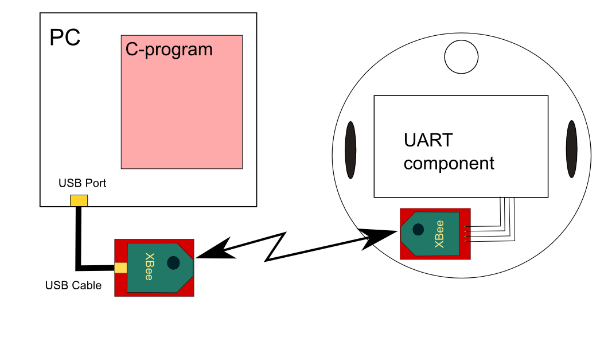
\includegraphics[width=0.65\textwidth]{zigbee.png}
	\caption{Verbinding tussen computer en robot}
	\label{fig:zigbee}
\end{figure}

De VHDL-code bestaat uit een Top-entity en Sub-entities;


\subsection{Top-entity}.

We willen ervoor zorgen dat de ontvangen bits worden getoond op de LEDs en de bits die verzonden moeten worden door de robot, verzonden worden door middel van de switches.
De bits die worden verzonden en ontvangen worden gebufferd in een 8-bit register en met behulp van flag flip-flops wordt de status van de 8-bit register bijgehouden.
Het verzenden van de bits begint als de write-data '1' is.
De ontvangen bits worden verwijderd als read-data '1' is.
Verder is er nog een 50MHz klok aanwezig.

\subsection{Sub-entities;}

Er zijn vier sub-entities, namelijk;

\begin{itemize}
\item  \textbf{Baud rate generator}\\
\newline
De baud rate generator zorgt ervoor dat er nauwkeurig wordt bijgehouden welke bits er binnenkomen.

\item \textbf{UART receiver}\\

De UART receiver bevat een FSM die bestaat uit vier statussen namelijk; idle, start, data en stop.
Hoe de FSM werkt, is afhankelijk van de kloksignalen die deze binnenkrijgt van de baud rate generator en de status van het 'rx' signaal.
De FSM begint in de idle status als 'rx' signaal 1 heeft.
Als rx vervolgens signaal 0 krijgt, gaat de FSM in de start status en begint het de pulsen te tellen.
Er zijn twee soorten tellers, \textit{n} en \textit{s}.
De eerste houdt het aantal pulsen bij, de tweede het ontvangen aantal data bits.
De ontvangen bits worden verplaatst naar een 8-bit register.
Als alles is afgerond, wordt het ontvangen bit gekopieerd naar de buffer register, waar op hetzelfde moment de flag flip-flop wordt ingesteld.
 
 \item \textbf{UART transmitter}\\

 De UART transmitter is een register die data bits op een bepaald tempo verplaatst.
Dit tempo wordt beïnvloed door de pulsen van de baud rate generator.
Als het overdracht proces van één data status is voltooid, wordt de flag flip-flop hierdoor gereset
 
 \item \textbf{Buffer register met flag flip-flops}\\

 De buffer register zorgt voor een link tussen het UART sub-systeem en het hoofdsysteem.
Een flag flip-flop houdt bij of de buffer register, vol of leeg is.\\

Als de UART receiver de ontvangen bit doorgeeft, geeft de flag flip-flop weer dat de buffer register gelezen is door het hoofdsysteem en dat die nu opnieuw ingesteld kan worden.\\

Als voor de UART transmitter de flag flip-flop aangeeft dat de buffer register de juiste data bevat om verzonden te worden, dan zal de UART transmitter op de actieve status van de flip-flop reageren en beginnen met verzenden.
De data van de buffer register wordt gekopieerd naar de UART transmitter en als deze vervolgens klaar is met het proces zal de flag flip-flop gereset worden, waarna er weer nieuwe data kan worden ontvangen 
 
\end{itemize}
De C-code die voor de communicatie geschreven moest worden, moet er voor zorgen dat er vanuit de C-code gecommuniceerd kan worden met de VHDL-code op de robot.
Via de 7-segmentdisplay kan er gezien worden wat er vanaf de computer naar de robot wordt verzonden. Éen uitgebreide uitleg hierover staat in hoofdstuk \ref{ch:sseg}.


\section{Implementatie}
Voordat de XBee modules met elkaar kunnen communiceren moeten ze eerst met elkaar worden geconfigureerd, zodat ze dezelfde unieke instellingen hebben.
Als dit niet wordt gedaan is het mogelijk dat andere XBee modules gaan communiceren met andere modules terwijl dit niet de bedoeling is.

De XBee modules bevatten een aantal instelpunten die ervoor zorgen dat er onderscheidt kan worden gemaakt tussen de verschillende XBee modules.
De belangrijkste hiervan zullen verder uitgelicht worden;

\subsection{Channel settings}
De XBee modules kunnen op zestien verschillende frequentiebreedtes werken, van 11(0x0B) tot 26 (0x1A).
Als er onderscheid moet worden gemaakt tussen XBee modules in de omgeving is het handig om deze op een andere frequentiebreedte te zetten.\\

\subsection{Pan-Id}
Als er meerdere XBee modules op dezelfde frequentiebreedte zitten kan er nog steeds onderscheid worden gemaakt tussen de XBee modules door middel van \textit{Pan-ID}.
Deze bestaat uit een 16-bits nummer.
Door op beide XBee modules de \textit{Pan-ID}  met hetzelfde nummer in te stellen, kan er alleen nog maar gecommuniceerd worden met de XBee modules die hetzelfde \textit{Pan-ID} hebben.

\subsection{My-ID;}
Het is mogelijk dat er meerdere XBee modules hetzelfde\textit{ Pan-Id} hebben.
Er moet daarom ook nog onderscheid kunnen worden gemaakt tussen de XBee modules met hetzelfde \textit{Pan-Id}.
Dit kan worden gedaan door \textit{My-Id} van de ene XBee modules, in te stellen in \textit{DL} van de andere XBee module, als je dit ook voor de andere XBee module doet, kan er alleen nog maar gecommuniceerd worden tussen deze XBees.


Voor de VHDL-code, de C-code en de instellingen van de XBee module zie bijlage; \ref{app:communicatie}

\section{Test}

We hebben de draadloze verbinding tussen de computer en de robot kunnen testen door te kijken of we ASCII-karakters(elk ASCII-karakter heeft zijn eigen 7-bit code) van de computer naar de robot konden sturen en vervolgens te kijken of deze in de juiste led volgorde op de robot verschenen. De meest rechter led indiceert de eerste bit. Vervolgens hebben we geprobeerd om vanaf de robot naar de computer bits te sturen, waarna er op de computer ASCII-karakters verschenen.

Daarna zijn we gaan kijken of we de robot konden laten rijden als we vanaf de computer één bepaalde bit zouden sturen. Hiervoor moesten we eerst in de VHDL-code van de robot aangeven welke bit zou staan voor het vooruit rijden. Zie hiervoor bijlage \ref{tab:comProtocol}Door deze bit te verzenden naar de robot en te aanschouwen of deze daadwerkelijk zou gaan vooruitrijden, konden we kijken of de draadloze communicatie tussen de XBee module van de computer en de XBee module van de robot goed werkte.

\section{Discussie}

Het draadloos communiceren van de XBee's werkte zeer goed.

Wat wellicht een probleem kan zijn, is dat toevallig mensen dezelfde instellingen hebben gekozen waardoor er tussen verschillende groepen gecommuniceerd wordt, wat zeker niet de bedoeling is.
Dit is echter bij ons niet het geval geweest.

\end{document}